% MICRO 2026 Survey Paper - ML Performance Models
% Using MICRO 59 ACM sigconf template
% Last compiled: 2026-02-07 (rebuild triggered)

%%
%% For submission and review of your manuscript please change the
%% command to \documentclass[manuscript, screen, review]{acmart}.
%%
\documentclass[sigconf, screen, review]{acmart}

%%
%% \BibTeX command to typeset BibTeX logo in the docs
\AtBeginDocument{%
  \providecommand\BibTeX{{%
    Bib\TeX}}}

%% Rights management information - for submission
\setcopyright{none}
\copyrightyear{2026}
\acmYear{2026}
\acmDOI{XXXXXXX.XXXXXXX}

%% Conference information
\acmConference[MICRO 2026]{The 59th IEEE/ACM International Symposium on Microarchitecture}{November 2026}{Austin, TX, USA}
\acmISBN{978-X-XXXX-XXXX-X/XX/XX}

%% Disable ACM reference format printing for submission
\settopmatter{printfolios=true}
\settopmatter{printacmref=false}

%% Additional packages (acmart already loads amsmath, amsfonts, amssymb, booktabs)
\usepackage{multirow}
\usepackage{tikz}
\usetikzlibrary{shapes.geometric,arrows.meta,positioning,fit,backgrounds}

% Custom commands
\newcommand{\todo}[1]{\textcolor{red}{[TODO: #1]}}

\begin{document}

\title{A Survey of High-Level Modeling and Simulation Methods for Modern Machine Learning Workloads}
\subtitle{\normalsize{MICRO 2026 Submission
    \textbf{\#NaN} -- Confidential Draft -- Do NOT Distribute!!}}

%%
%% The abstract is a short summary of the work to be presented in the
%% article.

%%%%%% -- PAPER CONTENT STARTS-- %%%%%%%%

\begin{abstract}
Machine learning-based performance modeling has emerged as a powerful alternative to traditional analytical models and cycle-accurate simulators for predicting computer system behavior.
This survey focuses specifically on \emph{ML techniques} for performance prediction across CPUs, GPUs, accelerators, and distributed systems, covering over 60 papers from architecture and ML venues published between 2016--2026.
We position traditional analytical models (Timeloop, MAESTRO) and simulators (gem5, GPGPU-Sim) as \emph{baselines} that ML approaches aim to replace or augment.
We organize ML approaches along three primary dimensions---modeling technique, target hardware, and input representation---while additionally characterizing papers by workload coverage, prediction targets, accuracy metrics, and evaluation scope.
Our analysis reveals that specialized ML models achieve remarkable accuracy---below 5\% error for narrow domains---while general-purpose models trade accuracy for broader applicability.
Transfer learning and meta-learning techniques increasingly enable adaptation to new hardware with minimal profiling, addressing the challenge of hardware diversity.
We identify key open challenges including benchmark diversity, cross-platform generalization, and integration with compiler and architecture exploration workflows.
Hybrid approaches combining analytical structure with learned components represent the most promising direction, offering both interpretability and accuracy.
This survey provides practitioners guidance for selecting appropriate ML techniques and researchers a roadmap for advancing the field.
\end{abstract}

%%
%% Keywords
\keywords{machine learning, performance modeling, computer architecture, neural networks, survey}

\maketitle

% ==============================================================================
% INTRODUCTION
% ==============================================================================
\section{Introduction}
\label{sec:introduction}

Performance modeling is fundamental to computer architecture research and development.
Architects rely on accurate performance predictions to navigate vast design spaces, optimize hardware-software co-design, and make informed decisions about resource allocation.
Traditional approaches---analytical models~\cite{williams2009roofline} and cycle-accurate simulators~\cite{binkert2011gem5}---have served the community well, but face growing challenges as workloads and hardware become increasingly complex.
Analytical models often oversimplify system behavior, while simulators can require hours or days to evaluate a single design point, making exhaustive exploration impractical.

The rise of deep learning workloads has intensified these challenges.
Modern neural networks exhibit diverse computational patterns---from dense matrix operations in transformers to sparse irregular accesses in graph neural networks---that stress traditional modeling assumptions.
Simultaneously, hardware diversity has exploded: GPUs, TPUs, custom accelerators, and multi-device distributed systems each present unique performance characteristics that resist unified analytical treatment.
This complexity has motivated a new generation of \emph{machine learning-based} performance models that learn predictive functions directly from profiling data.

ML-based performance modeling has emerged as a compelling alternative.
Learned models can capture complex, non-linear relationships between workload characteristics and hardware behavior that elude closed-form analysis.
Recent work demonstrates remarkable accuracy: NeuSight~\cite{neusight2025} achieves 2.3\% error predicting GPT-3 latency on H100 GPUs, while nn-Meter~\cite{nnmeter2021} reaches 99\% accuracy for edge device latency prediction.
Beyond accuracy, these approaches offer practical benefits: models trained on one platform can transfer to new hardware with minimal adaptation~\cite{litepred2024}, and inference-time predictions complete in milliseconds rather than hours.

This survey provides a comprehensive analysis of ML-based performance modeling techniques for computer architecture.
We focus specifically on \emph{learned} models that acquire predictive capability from data, positioning traditional analytical and simulation approaches as baselines that contextualize ML advances.
We make the following contributions:
\begin{itemize}
    \item A \textbf{taxonomy} organizing ML approaches along three primary dimensions (modeling technique, target hardware, input representation), with additional characterization by workload coverage, prediction targets, and accuracy.
    \item A \textbf{systematic survey} of over 60 ML-based performance modeling papers from architecture venues (MICRO, ISCA, HPCA, ASPLOS) and ML venues (MLSys, NeurIPS, ICML) published between 2016--2026.
    \item A \textbf{comparative analysis} examining trade-offs between accuracy, training cost, generalization, and interpretability across ML approaches.
    \item An identification of \textbf{open challenges} including data scarcity, cross-platform generalization, and integration with design automation flows.
\end{itemize}

The remainder of this paper is organized as follows.
Section~\ref{sec:background} provides background on traditional performance modeling and relevant ML techniques.
Section~\ref{sec:taxonomy} presents our classification taxonomy.
Section~\ref{sec:survey} surveys approaches organized by target hardware platform.
Section~\ref{sec:comparison} offers comparative analysis across key dimensions.
Section~\ref{sec:challenges} discusses open challenges and future directions.
Section~\ref{sec:evaluation} presents hands-on reproducibility evaluations of representative tools.
Section~\ref{sec:conclusion} concludes.

Figure~\ref{fig:timeline} illustrates the evolution of ML-based performance modeling, showing how techniques have progressed from simple regression models to sophisticated hybrid approaches achieving sub-5\% accuracy.

\begin{figure}[t]
\centering
\resizebox{\columnwidth}{!}{%
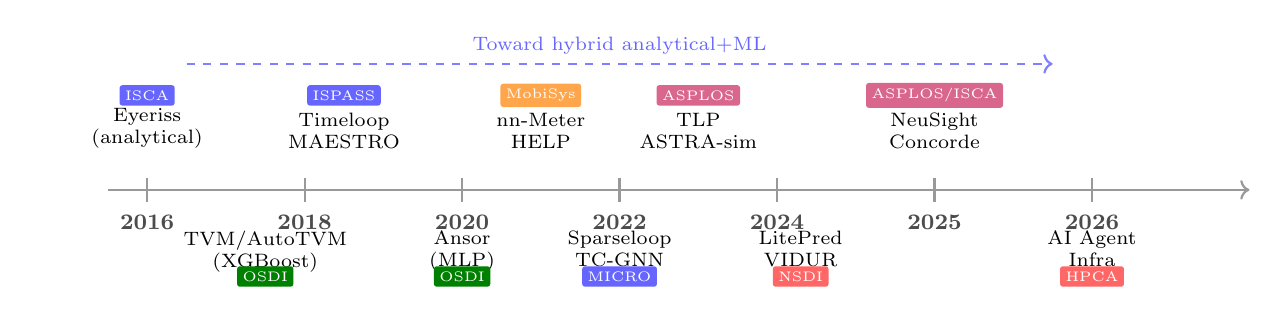
\begin{tikzpicture}[
    node distance=0.3cm,
    yearnode/.style={font=\footnotesize\bfseries, text=black!70},
    eventnode/.style={font=\scriptsize, text width=2.8cm, align=center},
    catnode/.style={font=\tiny, text=white, rounded corners=1pt, inner sep=2pt}
]
% Timeline base
\draw[thick, ->, black!40] (0,0) -- (14.5,0);

% Year markers
\foreach \x/\year in {0.5/2016, 2.5/2018, 4.5/2020, 6.5/2022, 8.5/2024, 10.5/2025, 12.5/2026} {
    \draw[thick, black!40] (\x,-0.15) -- (\x,0.15);
    \node[yearnode, below] at (\x,-0.2) {\year};
}

% Events - staggered heights to avoid overlap
% 2016-2017: Foundation
\node[eventnode, above] at (0.5,0.4) {Eyeriss\\(analytical)};
\node[catnode, fill=blue!60] at (0.5,1.2) {ISCA};

% 2018: TVM
\node[eventnode, below] at (2.0,-0.4) {TVM/AutoTVM\\(XGBoost)};
\node[catnode, fill=green!50!black] at (2.0,-1.1) {OSDI};

% 2019: Timeloop, MAESTRO
\node[eventnode, above] at (3.0,0.4) {Timeloop\\MAESTRO};
\node[catnode, fill=blue!60] at (3.0,1.2) {ISPASS};

% 2020: Ansor
\node[eventnode, below] at (4.5,-0.4) {Ansor\\(MLP)};
\node[catnode, fill=green!50!black] at (4.5,-1.1) {OSDI};

% 2021: nn-Meter, HELP
\node[eventnode, above] at (5.5,0.4) {nn-Meter\\HELP};
\node[catnode, fill=orange!70] at (5.5,1.2) {MobiSys};

% 2022: Sparseloop, GNN
\node[eventnode, below] at (6.5,-0.4) {Sparseloop\\TC-GNN};
\node[catnode, fill=blue!60] at (6.5,-1.1) {MICRO};

% 2023: TLP, ASTRA-sim
\node[eventnode, above] at (7.5,0.4) {TLP\\ASTRA-sim};
\node[catnode, fill=purple!60] at (7.5,1.2) {ASPLOS};

% 2024: LitePred, VIDUR
\node[eventnode, below] at (8.8,-0.4) {LitePred\\VIDUR};
\node[catnode, fill=red!60] at (8.8,-1.1) {NSDI};

% 2025: NeuSight, Concorde, AMALI
\node[eventnode, above] at (10.5,0.4) {NeuSight\\Concorde};
\node[catnode, fill=purple!60] at (10.5,1.2) {ASPLOS/ISCA};

% 2026: AI Agent Analysis
\node[eventnode, below] at (12.5,-0.4) {AI Agent\\Infra};
\node[catnode, fill=red!60] at (12.5,-1.1) {HPCA};

% Trend arrow
\draw[thick, ->, blue!50, dashed] (1,1.6) -- (12,1.6);
\node[font=\scriptsize, text=blue!60, above] at (6.5,1.6) {Toward hybrid analytical+ML};

\end{tikzpicture}
}
\caption{Evolution of ML-based performance modeling (2016--2026). Early work used analytical models (Eyeriss, Timeloop); ML approaches began with simple regressors (TVM) and progressed to deep learning (Ansor, HELP), GNNs (TC-GNN), and transformers (TLP). Current state-of-the-art combines analytical structure with neural networks (NeuSight, Concorde). Recent work extends to AI agent infrastructure analysis.}
\label{fig:timeline}
\end{figure}

% ==============================================================================
% BACKGROUND
% ==============================================================================
\section{Background}
\label{sec:background}

\subsection{Traditional Performance Modeling}
\label{subsec:traditional-modeling}

Performance modeling traditionally relies on analytical models and cycle-accurate simulation, which serve as baselines for ML techniques.

\subsubsection{Analytical Models}

Analytical models express performance as closed-form functions.
The roofline model~\cite{williams2009roofline} bounds performance by $P = \min(\pi, \beta \cdot I)$, where $\pi$ is peak FLOPS, $\beta$ is memory bandwidth, and $I$ is operational intensity.
For DNN accelerators, Timeloop~\cite{timeloop2019} models data movement across memory hierarchies, MAESTRO~\cite{maestro2019} provides data-centric dataflow analysis, and Sparseloop~\cite{sparseloop2022} extends to sparse tensors with 2000$\times$ speedup over RTL.
Analytical models offer fast evaluation (microseconds) and interpretability, but require manual derivation per architecture and struggle with complex microarchitectural effects.

\subsubsection{Cycle-Accurate Simulation}

Simulators like gem5~\cite{binkert2011gem5} for CPUs and GPGPU-Sim~\cite{gpgpusim2009}/Accel-Sim~\cite{accelsim2020} for GPUs model hardware at register-transfer level, achieving 5--15\% accuracy.
However, simulating a single ResNet-50 inference may require hours.
ASTRA-sim~\cite{astrasim2023} uses analytical abstractions for distributed training but still struggles with the scale of modern workloads.

\subsubsection{The Modeling Gap}

Analytical models are fast but imprecise; simulators are accurate but slow.
ML-based models offer a middle path: learning complex relationships from profiling data while enabling millisecond-scale inference.

\subsection{Machine Learning Fundamentals}
\label{subsec:ml-fundamentals}

We briefly review ML techniques used in performance modeling.

\textbf{Classical ML.}
Tree-based ensembles (XGBoost, LightGBM) dominate when training data is limited ($<$10K samples), often outperforming deep learning in low-data regimes~\cite{nnmeter2021}.

\textbf{Deep Learning.}
MLPs learn hierarchical features through stacked transformations.
RNNs/LSTMs process sequential inputs but are increasingly replaced by attention-based models.

\textbf{Graph Neural Networks.}
GNNs update node representations by aggregating neighbor information:
$\mathbf{h}_v^{(k+1)} = \phi(\mathbf{h}_v^{(k)}, \bigoplus_{u \in \mathcal{N}(v)} \psi(\mathbf{h}_u^{(k)}, \mathbf{e}_{uv}))$.
DNN computation graphs naturally map to this representation, with operators as nodes and data dependencies as edges~\cite{granite2022}.

\textbf{Transformers.}
Self-attention enables long-range dependency modeling without sequential processing, capturing complex inter-operator interactions.

\textbf{Transfer Learning.}
Enables training on easily-profiled hardware and transferring to new platforms with limited data through fine-tuning, domain adaptation, or meta-learning~\cite{litepred2024}.

\subsection{Problem Formulation}
\label{subsec:problem-formulation}

Performance modeling maps workload $\mathcal{W}$ and hardware $\mathcal{H}$ to metric $y$: $\hat{y} = f(\mathcal{W}, \mathcal{H}; \theta)$.
Workloads are represented at operator-level (layer parameters), graph-level (computation graphs), IR-level (compiler representations), or trace-level (runtime behavior).
Hardware is characterized by specifications, performance counters, or learned embeddings.

\textbf{Prediction targets} include latency (execution time), throughput (samples/second), energy (Joules/inference), and memory footprint.
Multi-objective formulations enable Pareto-optimal design selection.

\textbf{Accuracy metrics} include MAPE (scale-invariant relative error), RMSE (penalizes large errors), and correlation coefficients (Pearson, Kendall's $\tau$) for ranking accuracy.

\textbf{Hardware targets} span CPUs (cache hierarchies, out-of-order execution), GPUs (SIMT, warp scheduling), accelerators (systolic arrays, dataflows), edge devices (power/memory constraints), and distributed systems (communication, synchronization).
This diversity motivates our taxonomy in Section~\ref{sec:taxonomy}.

% ==============================================================================
% TAXONOMY
% ==============================================================================
\section{Taxonomy}
\label{sec:taxonomy}

We organize the literature along three dimensions: hardware target, ML technique, and input representation.
Figure~\ref{fig:taxonomy-overview} illustrates how these dimensions intersect.
This framework helps researchers identify explored versus open combinations, and enables practitioners to match methods to their requirements.

\begin{figure}[t]
\centering
\resizebox{\columnwidth}{!}{%
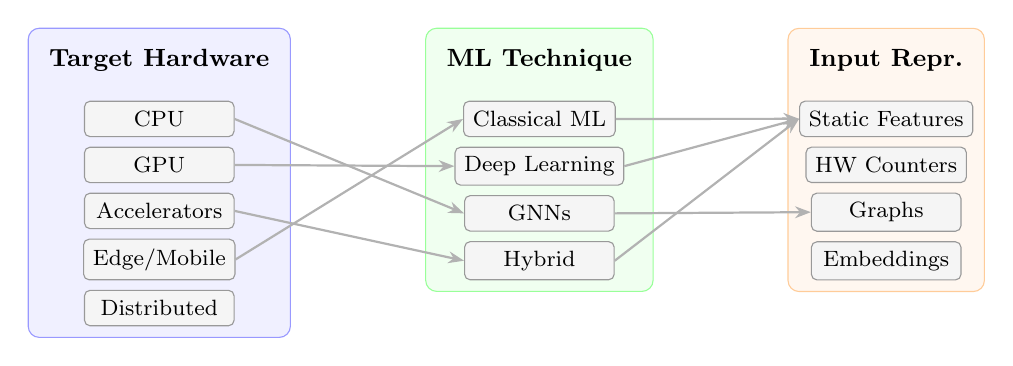
\begin{tikzpicture}[
    node distance=0.4cm and 0.6cm,
    dimbox/.style={rectangle, draw=black!70, fill=white, thick, minimum width=2.2cm, minimum height=0.6cm, font=\small},
    catbox/.style={rectangle, rounded corners=2pt, draw=black!40, fill=gray!8, minimum width=1.9cm, minimum height=0.45cm, font=\footnotesize},
    dimlabel/.style={font=\small\bfseries, text=black},
    arrow/.style={-{Stealth[length=2mm]}, thick, draw=black!50}
]

% === TARGET HARDWARE (Left column) ===
\node[dimlabel] (hw-label) at (0, 0) {Target Hardware};
\node[catbox, below=0.25cm of hw-label] (cpu) {CPU};
\node[catbox, below=0.12cm of cpu] (gpu) {GPU};
\node[catbox, below=0.12cm of gpu] (accel) {Accelerators};
\node[catbox, below=0.12cm of accel] (edge) {Edge/Mobile};
\node[catbox, below=0.12cm of edge] (dist) {Distributed};

% === ML TECHNIQUE (Middle column) ===
\node[dimlabel, right=2.0cm of hw-label] (ml-label) {ML Technique};
\node[catbox, below=0.25cm of ml-label] (classical) {Classical ML};
\node[catbox, below=0.12cm of classical] (deep) {Deep Learning};
\node[catbox, below=0.12cm of deep] (gnn) {GNNs};
\node[catbox, below=0.12cm of gnn] (hybrid) {Hybrid};

% === INPUT REPRESENTATION (Right column) ===
\node[dimlabel, right=2.0cm of ml-label] (inp-label) {Input Repr.};
\node[catbox, below=0.25cm of inp-label] (static) {Static Features};
\node[catbox, below=0.12cm of static] (counters) {HW Counters};
\node[catbox, below=0.12cm of counters] (graph) {Graphs};
\node[catbox, below=0.12cm of graph] (embed) {Embeddings};

% === Connecting arrows showing cross-dimensional relationships ===
% GPU -> Deep Learning (NeuSight, Habitat)
\draw[arrow, black!30] (gpu.east) -- (deep.west);
% Accelerators -> Hybrid (Timeloop, ArchGym)
\draw[arrow, black!30] (accel.east) -- (hybrid.west);
% Edge -> Classical ML (nn-Meter)
\draw[arrow, black!30] (edge.east) -- (classical.west);
% CPU -> GNN (GRANITE)
\draw[arrow, black!30] (cpu.east) -- (gnn.west);

% Deep Learning -> Static Features
\draw[arrow, black!30] (deep.east) -- (static.west);
% GNN -> Graph repr
\draw[arrow, black!30] (gnn.east) -- (graph.west);
% Classical ML -> Static/Counters
\draw[arrow, black!30] (classical.east) -- (static.west);
% Hybrid -> multiple
\draw[arrow, black!30] (hybrid.east) -- (static.west);

% === Background boxes for each dimension ===
\begin{scope}[on background layer]
    \node[fit=(hw-label)(cpu)(gpu)(accel)(edge)(dist), fill=blue!6, draw=blue!40, rounded corners=4pt, inner sep=4pt] {};
    \node[fit=(ml-label)(classical)(deep)(gnn)(hybrid), fill=green!6, draw=green!40, rounded corners=4pt, inner sep=4pt] {};
    \node[fit=(inp-label)(static)(counters)(graph)(embed), fill=orange!6, draw=orange!40, rounded corners=4pt, inner sep=4pt] {};
\end{scope}

\end{tikzpicture}%
}
\caption{Three-dimensional taxonomy for ML-based performance modeling. Arrows indicate common pairings observed in the literature (e.g., GPU models often use deep learning with static features).}
\label{fig:taxonomy-overview}
\end{figure}

\subsection{By Modeling Target}
\label{subsec:by-target}

The choice of hardware target fundamentally shapes model design, as different platforms exhibit distinct performance characteristics and modeling challenges.

\subsubsection{CPU Performance Modeling}

CPUs present complex modeling challenges due to deep out-of-order pipelines, sophisticated cache hierarchies, and branch prediction.
ML models for CPU performance must capture instruction-level parallelism, cache behavior, and memory access patterns.
Traditional approaches relied on microbenchmark-based linear regression~\cite{binkert2011gem5}, while recent work employs graph neural networks to model basic block throughput~\cite{granite2022}.
CPU modeling remains challenging due to the diversity of microarchitectures and the difficulty of capturing dynamic effects like branch misprediction and cache contention.

\subsubsection{GPU Performance Modeling}

GPUs dominate modern ML training and inference, making accurate GPU performance prediction critical.
GPU modeling must account for SIMT execution, warp scheduling, memory coalescing, and memory bandwidth limitations.
Early approaches used analytical roofline models~\cite{williams2009roofline}, but these struggle with the complex memory hierarchies and occupancy effects of modern GPUs.

ML-based GPU models have achieved remarkable accuracy.
NeuSight~\cite{neusight2025} introduces tile-based prediction that mirrors CUDA's execution model, achieving 2.3\% error on GPT-3 inference across H100, A100, and V100 GPUs.
Habitat~\cite{habitat2021} pioneered runtime-based cross-GPU prediction using wave scaling analysis.
These approaches demonstrate that learned models can capture GPU performance characteristics that elude analytical treatment.

\subsubsection{DNN Accelerator Modeling}

Custom DNN accelerators---including TPUs, NPUs, and systolic array designs---employ specialized dataflows optimized for matrix operations.
Modeling these devices requires understanding the interaction between dataflow, memory hierarchy, and tensor tiling.

Analytical frameworks like Timeloop~\cite{timeloop2019} and MAESTRO~\cite{maestro2019} provide systematic approaches for accelerator design space exploration.
Timeloop models data movement and compute utilization for any valid mapping of operations to hardware, achieving 5--10\% accuracy versus RTL simulation at 2000$\times$ speedup.
MAESTRO offers a data-centric perspective using intuitive dataflow directives.
Sparseloop~\cite{sparseloop2022} extends these frameworks to sparse tensor operations, critical for efficient transformer inference.

ML-based approaches complement analytical models by learning residual corrections or capturing effects not modeled analytically.
ArchGym~\cite{archgym2023} demonstrates that ML surrogate models can achieve 0.61\% RMSE while providing 2000$\times$ speedup over simulation, enabling rapid design space exploration for accelerator development.

\subsubsection{Edge and Mobile Device Modeling}

Edge devices impose strict power, memory, and latency constraints, making accurate prediction essential for deploying ML models on mobile phones, IoT devices, and embedded systems.
The diversity of edge hardware---spanning mobile CPUs, mobile GPUs, NPUs, and DSPs---creates significant challenges for cross-platform prediction.

nn-Meter~\cite{nnmeter2021} addresses this challenge through kernel-level prediction with adaptive sampling, achieving 99\% accuracy across mobile CPUs, GPUs, and Intel VPUs.
LitePred~\cite{litepred2024} extends this work with transfer learning, achieving 99.3\% accuracy across 85 edge platforms with less than one hour of adaptation per new device.
These results demonstrate that ML models can effectively generalize across the heterogeneous edge hardware landscape.

\subsubsection{Distributed System Modeling}

Multi-GPU and multi-node systems introduce communication overhead, synchronization barriers, and parallelism strategy choices that fundamentally change performance characteristics.
Distributed training performance depends on the interplay between compute, memory bandwidth, and network communication.

ASTRA-sim~\cite{astrasim2023} provides end-to-end distributed training simulation, modeling collective communication algorithms, network topology, and compute-communication overlap.
VIDUR~\cite{vidur2024} focuses specifically on LLM inference serving, capturing the unique characteristics of prefill and decode phases, KV cache management, and request scheduling.
These simulation frameworks achieve 5--15\% accuracy versus real clusters while enabling exploration of parallelization strategies at scale.

TrioSim~\cite{triosim2025} provides lightweight multi-GPU simulation for large-scale DNN workloads, complementing ASTRA-sim with faster execution through selective fidelity modeling.
Lumos~\cite{lumos2025} specifically targets LLM training performance prediction through trace-driven modeling, achieving 3.3\% error on H100 GPUs by capturing training-specific patterns including gradient accumulation, optimizer states, and activation checkpointing.

\subsection{By ML Technique}
\label{subsec:by-technique}

The choice of ML technique reflects trade-offs between accuracy, data efficiency, interpretability, and generalization capability.

\subsubsection{Classical Machine Learning}

Tree-based ensembles---random forests and gradient boosted trees (XGBoost, LightGBM)---remain highly effective for performance modeling, particularly in low-data regimes.
These methods handle non-linear relationships through recursive partitioning, provide feature importance rankings for interpretability, and require minimal hyperparameter tuning.

Classical ML models dominate when training data is limited ($<$10K samples) or when features are well-engineered.
nn-Meter~\cite{nnmeter2021} demonstrates that random forests achieve competitive accuracy with careful kernel-level feature engineering.
The ALCOP framework combines XGBoost with analytical pre-training, using analytical model predictions as features to accelerate autotuning convergence.

\subsubsection{Deep Learning}

Multi-layer perceptrons (MLPs) learn hierarchical feature representations without manual feature engineering.
MLPs are widely used as the prediction head in more complex architectures and as standalone models when sufficient training data is available.
NeuSight~\cite{neusight2025} uses MLPs to predict tile-level GPU utilization, learning complex interactions between tile parameters and hardware characteristics.

Recurrent neural networks (RNNs and LSTMs) process sequential inputs, making them suitable for modeling operator sequences in neural network execution.
However, sequential processing limits parallelization, and attention-based architectures increasingly replace RNNs for sequence modeling tasks.

\subsubsection{Graph Neural Networks}

Graph neural networks (GNNs) have emerged as particularly effective for performance modeling because computational graphs have natural graph structure.
Nodes represent operators with features (type, parameters, shapes), edges represent data dependencies with features (tensor dimensions, datatypes).
GNNs propagate performance-relevant information along these dependencies through message passing.

GRANITE~\cite{granite2022} applies GNNs to basic block throughput estimation, learning to predict CPU performance from instruction dependency graphs.
For DNN workloads, GNN-based models capture inter-operator interactions that flat feature representations miss.
The graph structure also enables natural handling of variable-size networks without padding or truncation.

\subsubsection{Hybrid Analytical+ML Models}

Hybrid approaches combine physics-based analytical models with learned components, achieving both interpretability and high accuracy.
The analytical component provides a strong prior based on hardware characteristics, while the ML component learns residual corrections and complex interactions.

This design philosophy has produced state-of-the-art results.
Analytical pre-training initializes ML models with reasonable predictions, reducing data requirements and improving convergence.
Physics-informed architectures incorporate analytical insights into model structure---NeuSight's tile-based prediction mirrors CUDA's execution model, providing inductive bias that improves generalization.
Residual learning trains ML models to predict the error of analytical models, combining analytical interpretability with ML's ability to capture unmodeled effects.

The latency predictor study~\cite{latencypredictorsnas2024} demonstrates that hybrid approaches with transfer learning achieve 22.5\% average improvement over baselines, with up to 87.6\% improvement on challenging cross-platform prediction tasks.

\subsection{By Input Representation}
\label{subsec:by-input}

Input representation determines what information the model can access and how effectively it can learn performance-relevant patterns.

\subsubsection{Static Features}

Static features derive from workload and hardware specifications without runtime measurement.
For DNN workloads, these include layer parameters (kernel size, channels, stride, batch size), tensor dimensions, and operator types.
Hardware specifications include core counts, memory sizes, bandwidth, and clock frequencies.

Static features enable prediction without profiling, supporting use cases like neural architecture search where thousands of candidate networks must be evaluated.
Feature engineering plays a critical role: effective representations capture computation-to-communication ratios, memory footprint estimates, and parallelization potential.

\subsubsection{Hardware Counters}

Performance counters provide runtime measurements of hardware behavior: cache miss rates, memory bandwidth utilization, instruction throughput, and stall cycles.
Counter-based models can capture dynamic effects invisible to static analysis, including contention, thermal throttling, and runtime scheduling decisions.

The primary limitation is that counter-based models require hardware execution, limiting their applicability for design space exploration or new architecture evaluation.
However, for optimizing existing deployments or debugging performance anomalies, counter-based models provide valuable insights that static approaches cannot match.

\subsubsection{Graph Representations}

Graph representations encode computational graphs with nodes representing operators and edges representing data dependencies.
Node features capture operator characteristics (type, parameters), while edge features encode tensor properties (shape, datatype, memory format).

Graph representations provide several advantages over flat feature vectors: they naturally handle variable-size networks, preserve structural information about operator interactions, and enable permutation-invariant predictions.
GNNs operating on these representations can learn which subgraph patterns indicate performance bottlenecks.

\subsubsection{Learned Embeddings}

Learned embeddings compress high-dimensional or categorical information into dense vector representations.
Hardware embeddings represent diverse devices as points in a learned feature space, enabling transfer learning across platforms.
Operator embeddings capture semantic similarities between operator types that may share performance characteristics.

HELP formulates hardware prediction as meta-learning, learning hardware embeddings that represent devices as black-box functions.
With just 10 measurement samples on a new device, HELP achieves accurate predictions by positioning the device appropriately in the learned embedding space.
This approach is particularly valuable for the fragmented edge hardware landscape, where collecting exhaustive training data for each device is impractical.

The comprehensive survey in Section~\ref{sec:survey} and Table~\ref{tab:survey-summary} illustrate the diversity of approaches across these taxonomy dimensions.

% ==============================================================================
% SURVEY OF APPROACHES
% ==============================================================================
\section{Survey of Approaches}
\label{sec:survey}

This section surveys ML-based performance modeling approaches organized by target hardware platform.
For each category, we examine the modeling challenges specific to that platform, describe representative techniques, and synthesize key findings across the literature.
Table~\ref{tab:survey-summary} provides a comprehensive comparison of the surveyed approaches.

\begin{table*}[t]
\centering
\caption{Summary of surveyed ML-based performance modeling approaches, organized by target hardware platform. $^*$PyTorchSim and TrioSim focus on simulation speedup rather than reporting absolute accuracy vs.\ real hardware; accuracy data not comparable to other entries.}
\label{tab:survey-summary}
\small
\begin{tabular}{llllll}
\toprule
\textbf{Paper} & \textbf{Platform} & \textbf{ML Technique} & \textbf{Prediction Target} & \textbf{Error} & \textbf{Key Innovation} \\
\midrule
\multicolumn{6}{l}{\textit{CPU Performance Modeling}} \\
GRANITE~\cite{granite2022} & CPU & GNN & Basic block throughput & 0.97 corr & Instruction graph encoding \\
Concorde~\cite{concorde2025} & CPU & Hybrid & CPI & 2\% & Compositional analytical-ML \\
gem5+ML~\cite{binkert2011gem5} & CPU & Hybrid & Execution time & 10--20\% & Simulation + learning \\
\midrule
\multicolumn{6}{l}{\textit{GPU Performance Modeling}} \\
NeuSight~\cite{neusight2025} & GPU & Hybrid MLP & Kernel/E2E latency & 2.3\% & Tile-based prediction \\
AMALI~\cite{amali2025} & GPU & Analytical & LLM inference & 23.6\% & Memory hierarchy modeling \\
Habitat~\cite{habitat2021} & GPU & MLP & Training time & 11.8\% & Wave scaling analysis \\
Accel-Sim~\cite{accelsim2020} & GPU & Simulation & Cycle-accurate & 10--20\% & SASS trace-driven \\
\midrule
\multicolumn{6}{l}{\textit{DNN Accelerator Modeling}} \\
Timeloop~\cite{timeloop2019} & NPU & Analytical & Latency/Energy & 5--10\% & Loop-nest DSE \\
MAESTRO~\cite{maestro2019} & NPU & Analytical & Latency/Energy & 5--15\% & Data-centric directives \\
Sparseloop~\cite{sparseloop2022} & NPU & Analytical & Sparse tensors & 5--10\% & Compression modeling \\
PyTorchSim~\cite{pytorchsim2025} & NPU & Simulation & Latency & N/A$^*$ & PyTorch 2 integration \\
ArchGym~\cite{archgym2023} & Multi & RL+Surrogate & Multi-objective & 0.61\% & ML-aided DSE \\
\midrule
\multicolumn{6}{l}{\textit{Edge Device Modeling}} \\
nn-Meter~\cite{nnmeter2021} & Edge & RF ensemble & Latency & $<$1\% & Kernel detection \\
LitePred~\cite{litepred2024} & Edge & VAE+MLP & Latency & 0.7\% & 85-platform transfer \\
HELP~\cite{help2021} & Multi & Meta-learning & Latency & 1.9\% & 10-sample adaptation \\
\midrule
\multicolumn{6}{l}{\textit{Distributed and LLM Systems}} \\
ASTRA-sim~\cite{astrasim2023} & Distributed & Simulation & Training time & 5--15\% & Collective modeling \\
TrioSim~\cite{triosim2025} & Multi-GPU & Simulation & DNN training & N/A$^*$ & Lightweight multi-GPU \\
Lumos~\cite{lumos2025} & Distributed & Trace-driven & LLM training & 3.3\% & H100 training modeling \\
VIDUR~\cite{vidur2024} & GPU cluster & Simulation & LLM serving & $<$5\% & Prefill/decode phases \\
\bottomrule
\end{tabular}
\end{table*}

\subsection{CPU Performance Modeling}
\label{subsec:cpu-modeling}

CPU performance modeling faces challenges from out-of-order execution, branch prediction, and deep cache hierarchies.
Traditional cycle-accurate simulation via gem5~\cite{binkert2011gem5} achieves 10--20\% accuracy but requires hours per DNN inference.

GRANITE~\cite{granite2022} uses GNNs to predict basic block throughput from instruction dependency graphs, achieving 0.97 Kendall's $\tau$ on x86 and generalizing across microarchitectures.
Concorde~\cite{concorde2025} advances hybrid modeling, achieving 2\% CPI error at five orders of magnitude faster than gem5 through compositional analytical-ML fusion.
Key remaining challenges include memory-bound execution (GRANITE focuses on compute-bound blocks), complex prefetchers, and optimized library code behavior.

\subsection{GPU Performance Modeling}
\label{subsec:gpu-modeling}

GPU modeling is challenging due to SIMT execution, complex memory hierarchies, and workload-dependent scheduling.
Cycle-accurate simulators (GPGPU-Sim~\cite{gpgpusim2009}, Accel-Sim~\cite{accelsim2020}) achieve 0.90--0.97 IPC correlation but suffer 1000--10000$\times$ slowdown.

\textbf{Learned models.}
Habitat~\cite{habitat2021} introduced wave scaling, decomposing execution into compute and memory components that scale with hardware parameters, achieving 11.8\% error across GPU generations.
NeuSight~\cite{neusight2025} advances this with tile-based prediction mirroring CUDA execution semantics, achieving 2.3\% error on GPT-3 inference (H100, A100, V100)---a 50$\times$ improvement over Habitat.

\textbf{Compiler cost models.}
TVM~\cite{tvm2018} and Ansor~\cite{ansor2020} use XGBoost/MLP models to guide autotuning, achieving $\sim$15\% MAPE.
The TenSet dataset (52M records) enables pre-trained models that accelerate autotuning 10$\times$.

\textbf{LLM inference.}
LLM execution exhibits distinct prefill (compute-bound) and decode (memory-bound) phases.
VIDUR~\cite{vidur2024} provides discrete-event simulation for serving systems, achieving $<$5\% error on end-to-end metrics.
AMALI~\cite{amali2025} reduces analytical modeling MAPE from 127\% to 24\% through improved memory hierarchy modeling.

\subsection{Accelerator Performance Modeling}
\label{subsec:accelerator-modeling}

DNN accelerators employ specialized dataflows and memory hierarchies optimized for tensor operations.

\textbf{Analytical modeling.}
Timeloop~\cite{timeloop2019} analytically computes data reuse, latency, and energy from loop-nest representations, achieving 5--10\% accuracy with 2000$\times$ speedup over RTL.
MAESTRO~\cite{maestro2019} offers data-centric dataflow directives; Sparseloop~\cite{sparseloop2022} extends to sparse tensors.

\textbf{ML-augmented design.}
ArchGym~\cite{archgym2023} connects ML optimization algorithms to simulators, with surrogate models achieving 0.61\% RMSE at 2000$\times$ speedup.
PyTorchSim~\cite{pytorchsim2025} integrates PyTorch 2 with NPU simulation supporting custom RISC-V ISA and systolic arrays.

Emerging accelerators (PIM, neuromorphic, analog) remain underexplored, with fundamentally different characteristics that existing frameworks do not address.

\subsection{Memory System Modeling}
\label{subsec:memory-modeling}

Memory increasingly dominates ML performance.
For DNN workloads, Timeloop~\cite{timeloop2019} computes exact access counts through data reuse analysis.
KV cache management has emerged as the dominant LLM serving challenge; vLLM's PagedAttention achieves 2--4$\times$ throughput through virtual memory techniques, while VIDUR~\cite{vidur2024} models cache allocation and eviction at the system level.

For distributed training, ASTRA-sim~\cite{astrasim2023} simulates collective communication algorithms, network topology, and compute-communication overlap, achieving 5--15\% error and enabling parallelization strategy exploration.

\subsection{Cross-Platform and Transfer Learning}
\label{subsec:transfer-learning}

Hardware diversity makes per-device training impractical.
HELP~\cite{help2021} formulates cross-hardware prediction as meta-learning, achieving 93.2\% accuracy with just 10 samples on new devices via MAML-style adaptation.
LitePred~\cite{litepred2024} scales to 85 edge devices using VAE-based intelligent sampling, achieving 99.3\% accuracy with under one hour of profiling per device.
Systematic evaluation~\cite{latencypredictorsnas2024} shows transfer learning provides 22.5\% average improvement, up to 87.6\% on challenging transfers.

Hybrid approaches like SynPerf combine analytical decomposition with learned components, achieving 6.1\% kernel-level error.
Key open challenges include transformer/MoE transfer (current work focuses on CNNs), cross-workload-type generalization, and continual learning for evolving software stacks

% ==============================================================================
% COMPARISON AND ANALYSIS
% ==============================================================================
\section{Comparison and Analysis}
\label{sec:comparison}

We now analyze trade-offs in accuracy, training cost, generalization, and interpretability.
Table~\ref{tab:comparison-summary} summarizes key dimensions.

\begin{table*}[t]
\centering
\caption{Comparative analysis of representative performance models---including ML-based and analytical/simulation approaches---across key dimensions. The Accuracy column reports the metric and value as given in each original work (e.g., MAPE, RMSE, Kendall's $\tau$, ranges).}
\label{tab:comparison-summary}
\small
\begin{tabular}{lcccccc}
\toprule
\textbf{Model} & \textbf{Accuracy (as reported)} & \textbf{Training Data} & \textbf{Adaptation Cost} & \textbf{Generalization} & \textbf{Interpretability} & \textbf{Inference Time} \\
\midrule
\multicolumn{7}{l}{\textit{Classical ML}} \\
nn-Meter~\cite{nnmeter2021} & $<$1\% MAPE & 1K/kernel & Hours/device & Device-specific & Medium & $<$1ms \\
XGBoost (TVM)~\cite{tvm2018} & 20\% MAPE & 10K+ & Online & Operator-level & Medium & $<$1ms \\
\midrule
\multicolumn{7}{l}{\textit{Deep Learning}} \\
NeuSight~\cite{neusight2025} & 2.3\% MAPE & 100K+ & Pre-trained & Cross-GPU & Low & $<$10ms \\
Habitat~\cite{habitat2021} & 11.8\% MAPE & Online profiling runs & None (requires GPU) & Cross-GPU & Medium & Per-kernel profiling \\
\midrule
\multicolumn{7}{l}{\textit{Graph Neural Networks}} \\
GRANITE~\cite{granite2022} & 0.97 $\tau$ & 10K+ & Hours & Cross-$\mu$arch & Low & $<$10ms \\
HELP~\cite{help2021} & 1.9\% MAPE & Meta-training & 10 samples & Cross-platform & Low & $<$10ms \\
\midrule
\multicolumn{7}{l}{\textit{Transfer Learning}} \\
LitePred~\cite{litepred2024} & 0.7\% MAPE & 85 platforms & 100 samples & 85+ devices & Low & $<$1ms \\
\midrule
\multicolumn{7}{l}{\textit{Hybrid Analytical+ML}} \\
Timeloop~\cite{timeloop2019} & 5--10\% & Arch spec & None & Any accelerator & High & $\mu$s \\
ArchGym~\cite{archgym2023} & 0.61\% RMSE & Simulation & Surrogate training & Architecture-specific & Medium & ms \\
VIDUR~\cite{vidur2024} & $<$5\% & Kernel profiles & Per-model & LLM-specific & High & ms \\
\bottomrule
\end{tabular}
\end{table*}

\noindent\textit{Note: Accuracy figures are reported as stated in original papers. Direct comparison is limited by differences in benchmarks, workloads, hardware targets, and evaluation protocols.}

\subsection{Accuracy vs. Training Cost}
\label{subsec:accuracy-cost}

Data collection cost varies dramatically: profiling-based methods (nn-Meter) require $\sim$1,000 samples/kernel; transfer learning (HELP, LitePred) reduces this to 10--100 samples.
Simulation-based training (ArchGym on Timeloop) avoids hardware entirely.

We observe three accuracy tiers: (1) Specialized models ($<$5\% error): nn-Meter, NeuSight, LitePred on narrow domains; (2) General-purpose (5--15\%): Habitat, Timeloop, MAESTRO; (3) Compiler cost models (15--25\%): TVM/AutoTVM, prioritizing ranking over absolute accuracy.
Accuracy requirements are use-case dependent---NAS tolerates 10--15\% error while hardware procurement demands $<$5\%.

\subsection{Generalization Capabilities}
\label{subsec:generalization}

\textbf{Workload generalization.}
GNN-based approaches (GRANITE~\cite{granite2022}) generalize via compositional learning, but cross-workload-type transfer (CNN$\rightarrow$transformer) remains challenging.
NeuSight~\cite{neusight2025} addresses this through diverse operator training.

\textbf{Hardware generalization.}
Three approaches show promise: meta-learning (HELP~\cite{help2021} with hardware embeddings), feature-based transfer (LitePred~\cite{litepred2024} achieving 92.1\% zero-shot accuracy), and analytical decomposition (Habitat~\cite{habitat2021} separating compute/memory components).

\textbf{Temporal generalization} as software evolves remains underexplored; continual learning for evolving stacks is an open direction.

\subsection{Interpretability}
\label{subsec:interpretability}

Analytical models (Timeloop, MAESTRO) provide full interpretability with actionable bottleneck identification.
Classical ML offers feature importance; deep learning is largely opaque.
Hybrid approaches (NeuSight, VIDUR) balance interpretability and accuracy by combining analytical structure with learned residuals, enabling ``what-if'' analysis.

% ==============================================================================
% OPEN CHALLENGES
% ==============================================================================
\section{Open Challenges and Future Directions}
\label{sec:challenges}

\subsection{Data Availability and Quality}
\label{subsec:data-challenges}

Existing datasets predominantly cover CNNs; transformers, MoE, and diffusion models remain underrepresented.
Hardware diversity creates bottlenecks---LitePred covers 85 devices but the landscape spans hundreds.
Measurement noise from thermal throttling and OS scheduling affects reliability; standardized protocols would improve comparability.

\subsection{Model Generalization}
\label{subsec:generalization-challenges}

Cross-workload generalization (CNN$\rightarrow$transformer) fails due to different computational patterns.
Cross-hardware transfer~\cite{litepred2024,help2021} shows promise for related platforms but cross-family prediction (GPU$\rightarrow$TPU) remains elusive.
Distribution shift from software evolution invalidates models; continual learning is underexplored.

\subsection{Integration with Design Flows}
\label{subsec:integration-challenges}

Compiler integration (TVM, Ansor) needs uncertainty quantification to improve exploration-exploitation trade-offs.
Architecture exploration (ArchGym) requires active learning for sample efficiency.
LLM serving needs real-time prediction within microseconds; VIDUR provides offline simulation but online adaptation is challenging.

\subsection{Research Opportunities}
\label{subsec:opportunities}

Five high-priority gaps:
(1) \textbf{Transformer cross-platform transfer}---current work focuses on CNNs; attention-based models have distinct memory patterns.
(2) \textbf{Uncertainty-aware autotuning}---calibrated confidence intervals could reduce measured evaluations.
(3) \textbf{Dynamic shape/sparse prediction}---existing models assume fixed inputs; LLM serving sees 128--128K tokens.
(4) \textbf{Unified energy-latency-memory prediction}---ML approaches focus on latency while edge/datacenter need energy.
(5) \textbf{Temporal robustness benchmarks}---no systematic evaluation of robustness to software evolution.

\subsection{Future Work: Toward Unified Tooling}
\label{subsec:unified-architecture}

No single tool addresses all needs; fragmentation forces practitioners to manage incompatible dependencies.
Key lessons from our evaluation: Docker-first deployment improves reproducibility; hybrid approaches combining analytical structure with learned components show best accuracy; portable model formats (ONNX) prevent versioning issues.
Future directions include unified workload representations and composable modeling engines with container isolation.

% ==============================================================================
% EXPERIMENTAL EVALUATION
% ==============================================================================
\section{Experimental Evaluation}
\label{sec:evaluation}

We conducted hands-on reproducibility evaluations of five representative tools using a 10-point rubric: Setup (3 pts: Docker availability, clean installation, quick start), Reproducibility (4 pts: reference outputs, determinism, examples), and Usability (3 pts: API clarity, interpretability, maintenance).
Table~\ref{tab:evaluation-summary} summarizes results.

\begin{table}[t]
\centering
\caption{Reproducibility evaluation scores (10-point rubric).}
\label{tab:evaluation-summary}
\small
\begin{tabular}{lcccc}
\toprule
\textbf{Tool} & \textbf{Setup} & \textbf{Reprod.} & \textbf{Usability} & \textbf{Total} \\
\midrule
Timeloop & 3 & 4 & 2 & 9/10 \\
ASTRA-sim & 2.5 & 3 & 3 & 8.5/10 \\
VIDUR & 2.5 & 3.5 & 3 & 9/10 \\
nn-Meter & 2 & 0 & 1 & 3/10 \\
NeuSight & 2 & 3 & 2.5 & 7.5/10 \\
\bottomrule
\end{tabular}
\end{table}

\textbf{Key findings.}
Docker-first tools (Timeloop, ASTRA-sim, VIDUR) scored 8.5+ by isolating dependencies; we executed all three on both x86\_64 and aarch64 without issues.
Timeloop provides reference outputs for all examples (Eyeriss, Simba) with deterministic results.
ASTRA-sim includes validated HGX-H100 configurations; VIDUR enables scheduler comparison (vLLM, Orca, Sarathi) without GPU hardware.
NeuSight's tile-based hybrid approach achieves 2.3\% error on LLM workloads.

\textbf{Critical anti-pattern.}
nn-Meter's pre-trained predictors fail with current scikit-learn due to pickle format changes---a cautionary example of ML model serialization fragility.
Projects should prefer portable formats (ONNX) or pin exact dependency versions.

\textbf{Best practices:} (1) Provide Docker images to isolate dependencies; (2) Document Python version requirements; (3) Include reference outputs for validation; (4) Use portable model formats; (5) Pin dependency versions.

% ==============================================================================
% CONCLUSION
% ==============================================================================
\section{Conclusion}
\label{sec:conclusion}

This survey analyzed over 60 papers on ML-based performance modeling for computer architecture.

\textbf{Key findings:}
(1) ML models achieve $<$5\% error on target domains (NeuSight 2.3\%, LitePred 0.7\%).
(2) Hybrid analytical+ML approaches dominate, combining interpretable structure with learned residuals (Concorde, AMALI, Lumos).
(3) Transfer learning enables 10--100 sample adaptation via meta-learning (HELP) and VAE sampling (LitePred).
(4) Kernel-level decomposition (nn-Meter) enables compositional predictions.
(5) LLM serving requires specialized modeling for prefill/decode phases and KV cache (VIDUR).

\textbf{Promising directions:}
Foundation models for performance prediction, uncertainty quantification for autotuning, temporal generalization via continual learning, multi-objective (latency/energy/memory) prediction, and emerging hardware (PIM, neuromorphic) support.

Machine learning has transformed performance modeling into a systematic discipline.
As ML workloads grow and hardware diversifies, accurate, generalizable models become critical for efficient system design.
This survey serves as both a reference for practitioners and a roadmap for researchers.

%%%%%%% -- PAPER CONTENT ENDS -- %%%%%%%%

%%
%% The next two lines define the bibliography style to be used, and
%% the bibliography file.
\bibliographystyle{ACM-Reference-Format}
\bibliography{references}

\end{document}
